\documentclass{beamer}
\usepackage[utf8]{inputenc}

\usetheme{Madrid}
\usecolortheme{default}
\usepackage{amsmath,amssymb,amsfonts,amsthm}
\usepackage{txfonts}
\usepackage{tkz-euclide}
\usepackage{listings}
\usepackage{adjustbox}
\usepackage{array}
\usepackage{tabularx}
\usepackage{gvv} 
\usepackage{lmodern}
\usepackage{circuitikz}
\usepackage{tikz}
\usepackage{graphicx}
\usepackage{comment}

\setbeamertemplate{page number in head/foot}[totalframenumber]

\usepackage{tcolorbox}
\tcbuselibrary{minted,breakable,xparse,skins}

\definecolor{bg}{gray}{0.95}
\DeclareTCBListing{mintedbox}{O{}m!O{}}{%
breakable=true,
listing engine=minted,
listing only,
minted language=#2,
minted style=default,
minted options={%
linenos,
gobble=0,
breaklines=true,
breakafter=,,
fontsize=\small,
numbersep=8pt,
#1},
boxsep=0pt,
left skip=0pt,
right skip=0pt,
left=25pt,
right=0pt,
top=3pt,
bottom=3pt,
arc=5pt,
leftrule=0pt,
rightrule=0pt,
bottomrule=2pt,
toprule=2pt,
colback=bg,
colframe=orange!70,
enhanced,
overlay={%
\begin{tcbclipinterior}
\fill[orange!20!white] (frame.south west) rectangle ([xshift=20pt]frame.north west);
\end{tcbclipinterior}},
#3,
}
\lstset{
language=C,
basicstyle=\ttfamily\small,
keywordstyle=\color{blue},
stringstyle=\color{orange},
commentstyle=\color{green!60!black},
numbers=left,
numberstyle=\tiny\color{gray},
breaklines=true,
showstringspaces=false,
}

\title
{2.8.25}
\date{September 19, 2025}
\author
{EE25BTECH11043 - Nishid Khandagre}

\begin{document}

\frame{\titlepage}

\begin{frame}{Question}
If $\vec{A}$, $\vec{B}$, $\vec{C}$ are mutually perpendicular vectors of equal magnitudes, show that $\vec{A}+\vec{B}+\vec{C}$ is equally inclined to $\vec{A}$, $\vec{B}$ and $\vec{C}$.
\end{frame}

\begin{frame}{Theoretical Solution}
Given:
\begin{align}
\vec{A}^\top \vec{B} &= 0 \\
\vec{B}^\top \vec{C} &= 0 \\
\vec{C}^\top \vec{A} &= 0
\end{align}

\begin{align}
\norm{\vec{A}} = \norm{\vec{B}} = \norm{\vec{C}} = k
\end{align}
\end{frame}

\begin{frame}{Theoretical Solution}
This implies:
\begin{align}
\vec{A}^\top \vec{A} &= \norm{\vec{A}}^2 = k^2 \\
\vec{B}^\top \vec{B} &= \norm{\vec{B}}^2 = k^2 \\
\vec{C}^\top \vec{C} &= \norm{\vec{C}}^2 = k^2
\end{align}

Let
\begin{align}
\vec{R} = \myvec{\vec{A} + \vec{B} + \vec{C}}
\end{align}

The cosine of the angle $\theta$ between two vectors $\vec{X}$ and $\vec{Y}$ is given by:
\begin{align}
\cos \theta = \frac{\vec{X}^\top \vec{Y}}{\norm{\vec{X}}\norm{\vec{Y}}}
\label{eq:equation}
\end{align}
\end{frame}

\begin{frame}{Theoretical Solution}
\begin{align}
\norm{\vec{R}}^2 &= \vec{R}^\top \vec{R} \\
&=\myvec{\vec{A} + \vec{B} + \vec{C}}^\top\myvec{\vec{A} + \vec{B} + \vec{C}} \\
&=\vec{A}^\top\vec{A}+\vec{A}^\top\vec{B}+\vec{A}^\top\vec{C}+\vec{B}^\top\vec{A}+\vec{B}^\top\vec{B}+\vec{B}^\top\vec{C}+\vec{C}^\top\vec{A}+\vec{C}^\top\vec{B}+\vec{C}^\top\vec{C} \\
&=\norm{\vec{A}}^2 + 0 + 0 + 0 + \norm{\vec{B}}^2 + 0 + 0 + 0 + \norm{\vec{C}}^2 \\
&=k^2 + k^2 + k^2\\
&=3k^2
\end{align}
Therefore, $\norm{\vec{R}} = \sqrt{3}k$.
\end{frame}

\begin{frame}{Theoretical Solution}
Now, let $\alpha$ be the angle between $\vec{R}$ and $\vec{A}$. using \eqref{eq:equation}
\begin{align}
\cos \alpha &= \frac{\vec{R}^\top \vec{A}}{\norm{\vec{R}} \norm{\vec{A}}} \\
&= \frac{\myvec{\vec{A} + \vec{B} + \vec{C}}^\top \vec{A}}{\norm{\vec{R}} \norm{\vec{A}}}   \\
&= \frac{\vec{A}^\top \vec{A} + \vec{B}^\top \vec{A} + \vec{C}^\top \vec{A}}{\norm{\vec{R}} \norm{\vec{A}}}   \\
&= \frac{\norm{\vec{A}}^2 + 0 + 0}{\norm{\vec{R}} \norm{\vec{A}}}  
\end{align}
\end{frame}

\begin{frame}{Theoretical Solution}
\begin{align}
&= \frac{k^2}{(\sqrt{3}k)(k)}  \\
&= \frac{k^2}{\sqrt{3}k^2}  \\
&= \frac{1}{\sqrt{3}}
\end{align}

Let $\beta$ be the angle between $\vec{R}$ and $\vec{B}$. using \eqref{eq:equation}
\begin{align}
\cos \beta &= \frac{\vec{R}^\top \vec{B}}{\norm{\vec{R}} \norm{\vec{B}}}  \\
&= \frac{\myvec{\vec{A} + \vec{B} + \vec{C}}^\top \vec{B}}{\norm{\vec{R}} \norm{\vec{B}}}   \\
&= \frac{\vec{A}^\top \vec{B} + \vec{B}^\top \vec{B} + \vec{C}^\top \vec{B}}{\norm{\vec{R}} \norm{\vec{B}}} 
\end{align}
\end{frame}

\begin{frame}{Theoretical Solution}
\begin{align}
&= \frac{0 + \norm{\vec{B}}^2 + 0}{\norm{\vec{R}} \norm{\vec{B}}}   \\
&= \frac{k^2}{(\sqrt{3}k)(k)}   \\
&= \frac{k^2}{\sqrt{3}k^2}   \\
&= \frac{1}{\sqrt{3}}
\end{align}
\end{frame}

\begin{frame}{Theoretical Solution}
Let $\gamma$ be the angle between $\vec{R}$ and $\vec{C}$. using \eqref{eq:equation}
\begin{align}
\cos \gamma &= \frac{\vec{R}^\top \vec{C}}{\norm{\vec{R}} \norm{\vec{C}}}\\
&= \frac{\myvec{\vec{A} + \vec{B} + \vec{C}}^\top \vec{C}}{\norm{\vec{R}} \norm{\vec{C}}}   \\
&= \frac{\vec{A}^\top \vec{C} + \vec{B}^\top \vec{C} + \vec{C}^\top \vec{C}}{\norm{\vec{R}} \norm{\vec{C}}}  
\end{align}
\end{frame}

\begin{frame}{Theoretical Solution}
\begin{align}
&= \frac{0 + 0 + \norm{\vec{C}}^2}{\norm{\vec{R}} \norm{\vec{C}}}   \\
&= \frac{k^2}{(\sqrt{3}k)(k)}   \\
&= \frac{k^2}{\sqrt{3}k^2}   \\
&= \frac{1}{\sqrt{3}}
\end{align}
Since $\cos \alpha = \cos \beta = \cos \gamma = \frac{1}{\sqrt{3}}$, it implies $\alpha = \beta = \gamma$.\\
Thus, $\vec{A}+\vec{B}+\vec{C}$ is equally inclined to $\vec{A}$, $\vec{B}$ and $\vec{C}$.
\end{frame}

\begin{frame}[fragile]
\frametitle{C Code}
\begin{lstlisting}
#include <stdio.h>
#include <math.h>

// Function to calculate the dot product of two 3D vectors
double dot_product(double v1x, double v1y, double v1z,
                   double v2x, double v2y, double v2z) {
    return v1x * v2x + v1y * v2y + v1z * v2z;
}

// Function to calculate the magnitude of a 3D vector
double magnitude(double vx, double vy, double vz) {
    return sqrt(vx * vx + vy * vy + vz * vz);
}
\end{lstlisting}
\end{frame}

\begin{frame}[fragile]
\frametitle{C Code}
\begin{lstlisting}
// Function to calculate the cosines of angles between (A+B+C) and A, B, C
// Arguments:
//   ax, ay, az: Components of vector A
//   bx, by, bz: Components of vector B
//   cx, cy, cz: Components of vector C
//   cos_angle_result: Pointer to an array to store the results
void calculate_angles_cosines(double ax, double ay, double az,
                              double bx, double by, double bz,
                              double cx, double cy, double cz,
                              double* cos_angle_result) {
    // Calculate the resultant vector R = A + B + C
    double rx = ax + bx + cx;
    double ry = ay + by + cy;
    double rz = az + bz + cz;
\end{lstlisting}
\end{frame}

\begin{frame}[fragile]
\frametitle{C Code}
\begin{lstlisting}
    // Calculate magnitudes
    double mag_A = magnitude(ax, ay, az);
    double mag_B = magnitude(bx, by, bz);
    double mag_C = magnitude(cx, cy, cz);
    double mag_R = magnitude(rx, ry, rz);

    // Calculate dot products
    double dot_R_A = dot_product(rx, ry, rz, ax, ay, az);
    double dot_R_B = dot_product(rx, ry, rz, bx, by, bz);
    double dot_R_C = dot_product(rx, ry, rz, cx, cy, cz);

    cos_angle_result[0] = dot_R_A / (mag_R * mag_A); 
    cos_angle_result[1] = dot_R_B / (mag_R * mag_B); 
    cos_angle_result[2] = dot_R_C / (mag_R * mag_C);
}
\end{lstlisting}
\end{frame}



\begin{frame}[fragile]
\frametitle{Python Code through shared output}
\begin{lstlisting}
import ctypes
import numpy as np
import matplotlib.pyplot as plt
from mpl_toolkits.mplot3d import Axes3D

# Load the shared library
lib_angles = ctypes.CDLL("./code4.so")

# Define the argument types and return type for the C function
lib_angles.calculate_angles_cosines.argtypes = [
    ctypes.c_double, ctypes.c_double, ctypes.c_double, # A_x, A_y, A_z
    ctypes.c_double, ctypes.c_double, ctypes.c_double, # B_x, B_y, B_z
    ctypes.c_double, ctypes.c_double, ctypes.c_double, # C_x, C_y, C_z
    ctypes.POINTER(ctypes.c_double * 3)                # Pointer to an array of 3 doubles for results
]
\end{lstlisting}
\end{frame}



\begin{frame}[fragile]
\frametitle{Python Code through shared output}
\begin{lstlisting}
lib_angles.calculate_angles_cosines.restype = None
# Define mutually perpendicular vectors of equal magnitude
magnitude = 5.0
A = np.array([magnitude, 0.0, 0.0])
B = np.array([0.0, magnitude, 0.0])
C = np.array([0.0, 0.0, magnitude])

# Resultant vector R = A + B + C
R = A + B + C
# Create a C array to hold the three cosine results
cos_angles_c_array = (ctypes.c_double * 3)()

# Call the C function
lib_angles.calculate_angles_cosines(
    A[0], A[1], A[2],
    B[0], B[1], B[2],
    C[0], C[1], C[2],
    ctypes.byref(cos_angles_c_array)
)
\end{lstlisting}
\end{frame}

\begin{frame}[fragile]
\frametitle{Python Code through shared output}
\begin{lstlisting}
# Retrieve the results from the C array
cos_theta_RA = cos_angles_c_array[0]
cos_theta_RB = cos_angles_c_array[1]
cos_theta_RC = cos_angles_c_array[2]

# Convert cosines to angles in degrees
theta_RA_deg = np.degrees(np.arccos(cos_theta_RA))
theta_RB_deg = np.degrees(np.arccos(cos_theta_RB))
theta_RC_deg = np.degrees(np.arccos(cos_theta_RC))

print(f"Vectors A = {A}, B = {B}, C = {C}")
print(f"Resultant vector R = A + B + C = {R}")
\end{lstlisting}
\end{frame}

\begin{frame}[fragile]
\frametitle{Python Code through shared output}
\begin{lstlisting}
print(f"Cosine of angle between R and A: {cos_theta_RA:.6f}")
print(f"Angle between R and A: {theta_RA_deg:.2f} degrees")
print(f"Cosine of angle between R and B: {cos_theta_RB:.6f}")
print(f"Angle between R and B: {theta_RB_deg:.2f} degrees")
print(f"Cosine of angle between R and C: {cos_theta_RC:.6f}")
print(f"Angle between R and C: {theta_RC_deg:.2f} degrees")

if np.isclose(theta_RA_deg, theta_RB_deg) and np.isclose(theta_RB_deg, theta_RC_deg):
    print("\nConclusion: The angles are approximately equal, showing that A+B+C is equally inclined to A, B, and C.")
else:
    print("\nConclusion: The angles are not equal. There might be an issue with the input vectors or calculation.")
\end{lstlisting}
\end{frame}

\begin{frame}[fragile]
\frametitle{Python Code through shared output}
\begin{lstlisting}
# --- Visualization ---
fig = plt.figure(figsize=(10, 8))
ax = fig.add_subplot(111, projection='3d')

origin = [0, 0, 0]

# Plot vectors A, B, C
ax.quiver(*origin, *A, color='r', linewidth=2, arrow_length_ratio=0.1, label='Vector A')
ax.quiver(*origin, *B, color='g', linewidth=2, arrow_length_ratio=0.1, label='Vector B')
ax.quiver(*origin, *C, color='b', linewidth=2, arrow_length_ratio=0.1, label='Vector C')

# Plot resultant vector R
ax.quiver(*origin, *R, color='purple', linewidth=3, arrow_length_ratio=0.08, label='Vector A+B+C')
\end{lstlisting}
\end{frame}

\begin{frame}[fragile]
\frametitle{Python Code through shared output}
\begin{lstlisting}
# Set labels and title
ax.set_xlabel('X-axis')
ax.set_ylabel('Y-axis')
ax.set_zlabel('Z-axis')
ax.set_title('Mutually Perpendicular Vectors and Their Sum')
ax.legend()

# Set limits for a better view
max_coord = max(np.max(np.abs(A)), np.max(np.abs(B)), np.max(np.abs(C)), np.max(np.abs(R))) * 1.2
ax.set_xlim([-max_coord, max_coord])
ax.set_ylim([-max_coord, max_coord])
ax.set_zlim([-max_coord, max_coord])

# Add grid
ax.grid(True)
plt.savefig("fig1.png") # Save the plot
plt.show()
\end{lstlisting}
\end{frame}

\begin{frame}[fragile]
\frametitle{Python Code}
\begin{lstlisting}
import numpy as np
import numpy.linalg as LA
import matplotlib.pyplot as plt
from mpl_toolkits.mplot3d import Axes3D # For 3D plotting

# --- 1. Define vectors A, B, C ---
# Mutually perpendicular vectors of equal magnitude
magnitude = 3.0 # You can change the magnitude
A = np.array([magnitude, 0.0, 0.0])
B = np.array([0.0, magnitude, 0.0])
C = np.array([0.0, 0.0, magnitude])

print(f"Given Vectors:")
print(f"A = {A}")
print(f"B = {B}")
print(f"C = {C}")
\end{lstlisting}
\end{frame}

\begin{frame}[fragile]
\frametitle{Python Code}
\begin{lstlisting}
# --- 2. Calculate the resultant vector R = A + B + C ---
R = A + B + C
print(f"\nResultant vector R = A + B + C = {R}")

# --- 3. Calculate angles using dot products ---
def angle_between_vectors(v1, v2):
    dot_product = np.dot(v1, v2)
    magnitude_v1 = LA.norm(v1)
    magnitude_v2 = LA.norm(v2)

    # Handle potential division by zero for zero vectors
    if magnitude_v1 < 1e-9 or magnitude_v2 < 1e-9:
        if magnitude_v1 < 1e-9 and magnitude_v2 < 1e-9:
            return 0.0 # Both are zero, angle is 0
        else:
            return np.pi / 2 # One is zero, other non-zero, angle is 90 degrees (pi/2 radians)
\end{lstlisting}
\end{frame}

\begin{frame}[fragile]
\frametitle{Python Code }
\begin{lstlisting}
    cosine_angle = dot_product / (magnitude_v1 * magnitude_v2)
    # Ensure cosine_angle is within [-1, 1] due to potential floating point inaccuracies
    cosine_angle = np.clip(cosine_angle, -1.0, 1.0)
    return np.arccos(cosine_angle) # Returns angle in radians

# Calculate angles
angle_RA_rad = angle_between_vectors(R, A)
angle_RB_rad = angle_between_vectors(R, B)
angle_RC_rad = angle_between_vectors(R, C)

angle_RA_deg = np.degrees(angle_RA_rad)
angle_RB_deg = np.degrees(angle_RB_rad)
angle_RC_deg = np.degrees(angle_RC_rad)

print("\n--- Calculated Angles ---")
print(f"Angle between R and A: {angle_RA_deg:.2f} degrees")
print(f"Angle between R and B: {angle_RB_deg:.2f} degrees")
print(f"Angle between R and C: {angle_RC_deg:.2f} degrees")
\end{lstlisting}
\end{frame}

\begin{frame}[fragile]
\frametitle{Python Code}
\begin{lstlisting}
# Conclusion
if np.isclose(angle_RA_deg, angle_RB_deg) and np.isclose(angle_RB_deg, angle_RC_deg):
    print("\nConclusion: The angles are approximately equal. This shows that A+B+C is equally inclined to A, B, and C.")
else:
    print("\nConclusion: The angles are not equal. Please check the input vectors to ensure they are mutually perpendicular and have equal magnitudes.")

# --- 5. Generate a 3D plot to visualize these vectors ---
fig = plt.figure(figsize=(10, 8))
ax = fig.add_subplot(111, projection='3d')

origin = [0, 0, 0]
\end{lstlisting}
\end{frame}

\begin{frame}[fragile]
\frametitle{Python Code }
\begin{lstlisting}
# Plot vectors A, B, C
ax.quiver(*origin, *A, color='r', linewidth=2, arrow_length_ratio=0.1, label='Vector A')
ax.quiver(*origin, *B, color='g', linewidth=2, arrow_length_ratio=0.1, label='Vector B')
ax.quiver(*origin, *C, color='b', linewidth=2, arrow_length_ratio=0.1, label='Vector C')

# Plot resultant vector R
ax.quiver(*origin, *R, color='purple', linewidth=3, arrow_length_ratio=0.08, label='Vector A+B+C')

# Set labels and title
ax.set_xlabel('X-axis')
ax.set_ylabel('Y-axis')
ax.set_zlabel('Z-axis')
ax.set_title('Mutually Perpendicular Vectors and Their Sum')
ax.legend()
\end{lstlisting}
\end{frame}

\begin{frame}[fragile]
\frametitle{Python Code (Direct) - Visualization}
\begin{lstlisting}[language=Python]
# Set limits for a better view
all_coords = np.concatenate((A, B, C, R))
max_coord = np.max(np.abs(all_coords)) * 1.2 # Add some padding
ax.set_xlim([-max_coord, max_coord])
ax.set_ylim([-max_coord, max_coord])
ax.set_zlim([-max_coord, max_coord])

# Add grid
ax.grid(True)

plt.savefig("fig2.png")
plt.show()

print("\nFigure saved as fig2.png")
\end{lstlisting}
\end{frame}

\begin{frame}{Plot by Python using shared output from C}
\begin{figure}[H]
        \centering
        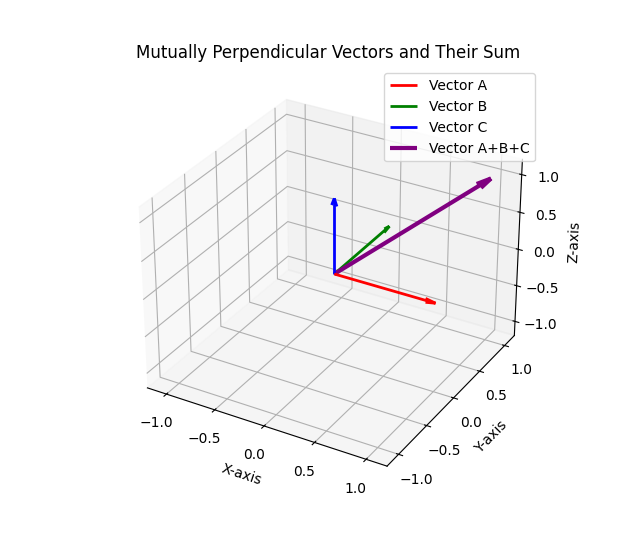
\includegraphics[width=0.8\columnwidth]{../figs/fig1.png}
        \caption{}
        \label{fig:1}
    \end{figure}
\end{frame}

 \begin{frame}{Plot by Python only}
\begin{figure}[H]
        \centering
        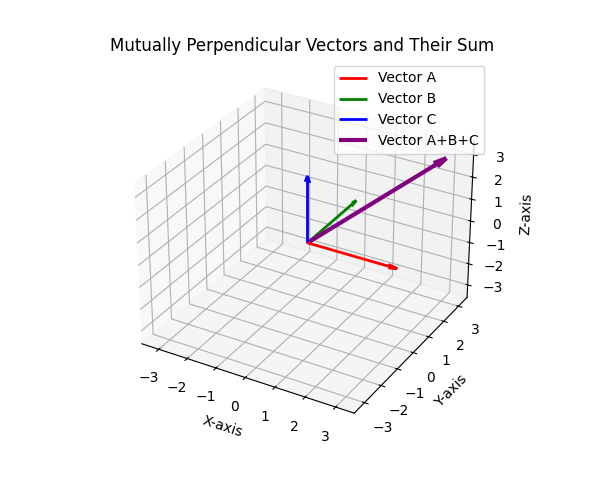
\includegraphics[width=0.8\columnwidth]{../figs/fig2.png}
        \caption{}
        \label{fig:2}
    \end{figure}
\end{frame}

\end{document}
